\paragraph{QuizziPedia::Front-End::Directives::MenuBarDirective}
\label{QuizziPedia::Front-End::Directives::MenuBarDirective}

\begin{figure}[ht]
	\centering
	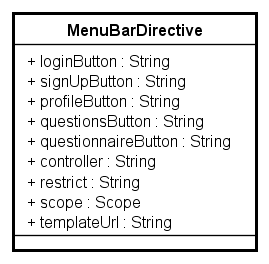
\includegraphics[scale=0.80,keepaspectratio]{UML/Classi/Front-End/QuizziPedia_Front-end_Directives_MenuBarDirective.png}
	\caption{QuizziPedia::Front-End::Directives::MenuBarDirective}
\end{figure} 
\FloatBarrier

\begin{itemize}
	\item \textbf{Descrizione}: rappresenta il menù, presente in ogni pagina dell'applicazione, generato in base agli oggetti passati nello \$scope isolato. Fornisce un pulsante per ogni oggetto ricevuto come parametro, ogni pulsante viene rappresentato con un’icona e con un testo. Al click di un pulsante viene invocata la funzione ad esso associata;
	\item \textbf{Utilizzo}: viene utilizzato per realizzare il menù, presente in ogni pagina dell'applicazione, che permette all'utente di selezionare un'opzione in base al contesto in cui si trova:
		\begin{itemize}
			\item Autenticazione;
			\item Registrazione;
			\item Ricerca;
			\item Visualizzare il proprio profilo utente;
			\item Gestire le domande create;
			\item Gestire i questionari creati.
		\end{itemize}
	\item \textbf{Relazioni con altre classi}: 
	\begin{itemize}
		\item \textit{IN} \texttt{Index}: view generale dell'applicazione;
		\item \textit{IN} \texttt{SearchDirective}: directive che permette di effettuare la ricerca di utenti e questionari;
		\item \textit{IN} \texttt{LogoutController}: questa classe permette di gestire la pagina di logout;
		\item \textit{IN} \texttt{MenuBarController}: questa classe permette di gestire il menù fisso per ogni pagina;
	\end{itemize}
	\item \textbf{Attributi}: 
	\begin{itemize}
		\item \texttt{+ loginButton: String} \\ Attributo che viene utilizzato per visualizzare la giusta traduzione della \textit{label\ped{G}} per il bottone di link all'autenticazione, in italiano o in inglese;
		\item \texttt{+ signUpButton: String} \\ Attributo che viene utilizzato per visualizzare la giusta traduzione della \textit{label\ped{G}} per il bottone di link alla registrazione, in italiano o in inglese;
		\item \texttt{+ profileButton: String} \\ Attributo che viene utilizzato per visualizzare la giusta traduzione della \textit{label\ped{G}} per il bottone di link al profilo utente, in italiano o in inglese;
		\item \texttt{+ questionsButton: String} \\ Attributo che viene utilizzato per visualizzare la giusta traduzione della \textit{label\ped{G}} per il bottone di link alla gestione delle domande, in italiano o in inglese;
		\item \texttt{+ questionnaireButton: String} \\ Attributo che viene utilizzato per visualizzare la giusta traduzione della \textit{label\ped{G}} per il bottone di link alla gestione dei questionari, in italiano o in inglese;
		\item \texttt{+ controller: String} \\ Stringa contenente il nome del controller della direttiva;
		\item \texttt{+ restrict: String} \\ Stringa che permette di definire le modalità di inserimento della direttiva all'interno della pagina;
		\item \texttt{+ scope: Scope}: oggetto scope interno della direttiva, contiene le funzionalità per gestire i dati presenti all'interno;
		\item \texttt{+ templateUrl: String} \\ Stringa contenente il percorso del file \textit{HTML\ped{G}} che contiene la direttive.
	\end{itemize}
\end{itemize}

\paragraph{QuizziPedia::Front-End::Directives::NewQuestionButtonDirective}

\label{QuizziPedia::Front-End::Directives::NewQuestionButtonDirective}

\begin{figure}[ht]
	\centering
	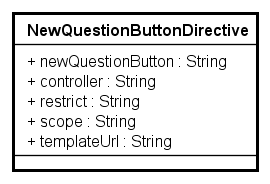
\includegraphics[scale=0.80,keepaspectratio]{UML/Classi/Front-End/QuizziPedia_Front-end_Directives_NewQuestionButtonDirective.png}
	\caption{QuizziPedia::Front-End::Directives::NewQuestionButtonDirective}
\end{figure} 
\FloatBarrier

\begin{itemize}
	\item \textbf{Descrizione}: rappresenta il componente grafico che permette all'utente di posizionarsi nella view di creazione di una nuova domanda;
	\item \textbf{Utilizzo}: viene utilizzato per permette all'utente di posizionarsi nella view di creazione di una nuova domanda;
	\item \textbf{Relazioni con altre classi}: 
	\begin{itemize}
		\item \textit{IN} \texttt{QuestionsManagementView}: view contenente l'elenco delle domande create; 
		\item \textit{IN} \texttt{NewQuestionsButtonsController}: questa classe permette di effettuare il redirect alla pagina di creazione nuova domanda;
		\item \textit{IN} \texttt{NewQuestionButtonsModelView}: classe di tipo modelview la cui istanzazione è contenuta all'interno della variabile di ambiente \$scope di \textit{Angular.js\ped{G}}. All'interno di essa sono presenti le variabili e i metodi necessari per il \textit{Two-Way Data-Binding\ped{G}} tra la directive \texttt{NewQuestionButtonsDirective} e il controller \texttt{NewQuestionsButtonController}; 
		\item \textit{IN} \texttt{LangModel}: rappresenta il modello delle informazioni per la giusta traduzione dell'applicazione.
	\end{itemize}
	\item \textbf{Attributi}: 
	\begin{itemize}
		\item \item {+ newQuestionButton: String} \\ Attributo che viene utilizzato per visualizzare la giusta traduzione della \textit{label\ped{G}} per il bottone di creazione di una nuova domanda, in italiano o in inglese;
		\item \texttt{+ controller: String} \\ Stringa contenente il nome del controller della direttiva;
		\item \texttt{+ restrict: String} \\ Stringa che permette di definire le modalità di inserimento della direttiva all'interno della pagina;
		\item \texttt{+ scope: Scope} \\ Oggetto scope interno della direttiva, contiene le funzionalità per gestire i dati presenti all'interno;
		\item \texttt{+ templateUrl: String} \\ Stringa contenente il percorso del file \textit{HTML\ped{G}} che contiene la direttive.
	\end{itemize}
\end{itemize}

\paragraph{QuizziPedia::Front-End::Directives::OneQuestionDirective}

\label{QuizziPedia::Front-End::Directives::OneQuestionDirective}

\begin{figure}[ht]
	\centering
	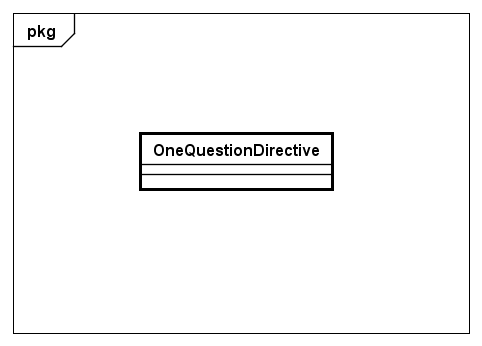
\includegraphics[scale=0.80,keepaspectratio]{UML/Classi/Front-End/QuizziPedia_Front-end_Directives_OneQuestionDirective.png}
	\caption{QuizziPedia::Front-End::Directives::OneQuestionDirective}
\end{figure} 
\FloatBarrier

\begin{itemize}
	\item \textbf{Descrizione}: rappresenta il componente grafico che visualizza all'utente l'anteprima della domanda che ha creato. Eseguendo l'azione di click sul pulsante di modifica sarà possibile modificare tale domanda. All'interno di QuestionsManagementsView verranno stampati a video tanti componenti quanti presenti nello \$scope isolato ad esso associato;
	\item \textbf{Utilizzo}: viene utilizzato per permettere all'utente di visualizzare le domande che ha creato;
	\item \textbf{Relazioni con altre classi}: 
	\begin{itemize}
		\item \textit{IN} \texttt{QuestionsManagementView}: view contenente l'elenco delle domande create;
		\item \textit{IN} \texttt{LangModel}: rappresenta il modello delle informazioni per la giusta traduzione dell'applicazione. 
	\end{itemize}
	\item \textbf{Attributi}: 
	\begin{itemize}
		\item \item {+ modifyButton: String} \\ Attributo che viene utilizzato per visualizzare la giusta traduzione della \textit{label\ped{G}} per il bottone di modifica della domanda, in italiano o in inglese.
	\end{itemize}
\end{itemize}

\paragraph{QuizziPedia::Front-End::Directives::QuestionTextDirective}

\label{QuizziPedia::Front-End::Directives::QuestionTextDirective}

\begin{figure}[ht]
	\centering
	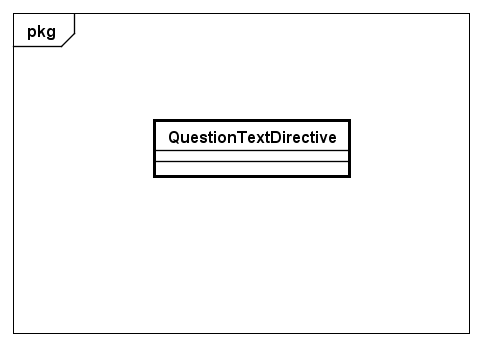
\includegraphics[scale=0.80,keepaspectratio]{UML/Classi/Front-End/QuizziPedia_Front-end_Directives_QuestionTextDirective.png}
	\caption{QuizziPedia::Front-End::Directives::QuestionTextDirective}
\end{figure} 
\FloatBarrier

\begin{itemize}
	\item \textbf{Descrizione}: rappresenta il componente grafico che permette all'utente di scrivere o modificare il testo di una domanda;
	\item \textbf{Utilizzo}: viene usato per permettere all'utente di scrivere o modificare il testo di una domanda;
	\item \textbf{Relazioni con altre classi}: 
	\begin{itemize}
		\item \textit{IN} \texttt{TrueFalseQuestionsView}: view contenente i campi per creare una domanda vero/falso; 
		\item \textit{IN} \texttt{MultipleQuestionsView}: view contenente i campi per creare una domanda a risposta multipla;
		\item \textit{IN} \texttt{ConnectionQuestionsView}: view contenente i campi per creare una domanda a collegamento;
		\item \textit{IN} \texttt{ImagesSortingQuestionsView}: view contenente i campi per creare una domanda a ordinamento immagini;
		\item \textit{IN} \texttt{StringsSortingQuestionsView}: view contenente i campi per creare una domanda a ordinamento stringhe;
		\item \textit{IN} \texttt{FillingQuestionsView}: view contenente i campi per creare una domanda a riempimento testo;
		\item \textit{IN} \texttt{ClickableAreaQuestionsView}: view contenente i campi per creare una domanda ad area cliccabile;
	\end{itemize}
	\item \textbf{Attributi}: 
	\begin{itemize}
		\item {+ questionText: String} \\ Attributo contenente il testo della domanda;
	\end{itemize}
\end{itemize}

\paragraph{QuizziPedia::Front-End::Directives::QuestionnaireDetailsDirective}

\label{QuizziPedia::Front-End::Directives::QuestionnaireDetailsDirective}

\begin{figure}[ht]
	\centering
	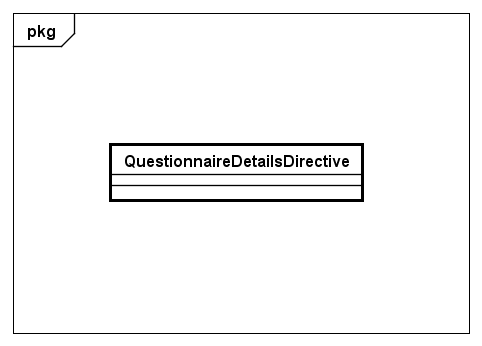
\includegraphics[scale=0.80,keepaspectratio]{UML/Classi/Front-End/QuizziPedia_Front-end_Directives_QuestionnaireDetailsDirective.png}
	\caption{QuizziPedia::Front-End::Directives::QuestionnaireDetailsDirective}
\end{figure} 
\FloatBarrier

\begin{itemize}
	\item \textbf{Descrizione}: rappresenta il componente grafico che permette all'utente di visualizzare la lista di questionari che può compilare. Ogni item di questa lista contiene:
		\begin{itemize}
			\item Nome del questionario;
			\item Autore del questionario;
			\item Argomento del questionario;
			\item Parole chiave del questionario;
		\end{itemize}
	Al verificarsi dell'evento click su un item della lista l'utente verrà indirizzato alla view per la compilazione del questionario selezionato;
	\item \textbf{Utilizzo}: viene utilizzato per permettere all'utente di visualizzare la lista di questionari che può compilare;
	\item \textbf{Relazioni con altre classi}: 
	\begin{itemize}
		\item \textit{IN} \texttt{UserView}: view contenente i dati personali dell'utente, le sue statistiche relative ai questionari e agli allenamenti effettuati e i questionari a cui è iscritto;
		\item \textit{IN} \texttt{QuestionnaireDetailsController}: questa classe permette di gestire i dettagli di un questionario;
		\item \textit{IN} \texttt{QuestionnaireDetailsModelView}: classe di tipo modelview la cui istanzazione è contenuta all'interno della variabile di ambiente \$scope di \texttt{Angular.js}. All'interno di essa sono presenti le variabili e i metodi necessari per il \textit{Two-Way Data-Binding\ped{G}} tra la view \texttt{UserView} e il controller \texttt{QuestionnaireDetailsController};
		\item \textit{IN} \texttt{LangModel}: rappresenta il modello delle informazioni per la giusta traduzione dell'applicazione. 
	\end{itemize}
	\item \textbf{Attributi}: 
	\begin{itemize}
		\item \texttt{+ questionnaireDetails: Object} \\ Oggetto contenente i seguenti campi dati: \texttt{name}, \texttt{author}, \texttt{topic} e \texttt{keywords};
		\item \texttt{+ compileButton: String} \\ Attributo che viene utilizzato per visualizzare la giusta traduzione della \textit{label\ped{G}} per il bottone di compilazione del questionario, in italiano o in inglese;
		\item \texttt{+ controller: String} \\ Stringa contenente il nome del controller della direttiva;
		\item \texttt{+ restrict: String} \\ Stringa che permette di definire le modalità di inserimento della direttiva all'interno della pagina;
		\item \texttt{+ scope: Scope} \\ Oggetto scope interno della direttiva, contiene le funzionalità per gestire i dati presenti all'interno;
		\item \texttt{+ templateUrl: String} \\ Stringa contenente il percorso del file \textit{HTML\ped{G}} che contiene la direttive.
	\end{itemize}
\end{itemize}

\paragraph{QuizziPedia::Front-End::Directives::QuestionnaireDoneDetailsDirective}

\label{QuizziPedia::Front-End::Directives::QuestionnaireDoneDetailsDirective}

\begin{figure}[ht]
	\centering
	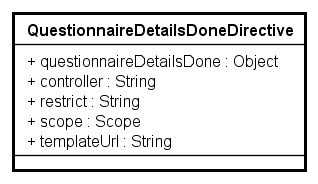
\includegraphics[scale=0.80,keepaspectratio]{UML/Classi/Front-End/QuizziPedia_Front-end_Directives_QuestionnaireDetailsDoneDirective.png}
	\caption{QuizziPedia::Front-End::Directives::QuestionnaireDetailsDoneDirective}
\end{figure} \FloatBarrier

\begin{itemize}
	\item \textbf{Descrizione}: rappresenta il componente grafico che permette all'utente di visualizzare la lista di questionari che ha già compilato e di conseguenza vederne le valutazioni. Ogni item di questa lista contiene:
	\begin{itemize}
		\item Nome del questionario;
		\item Autore del questionario;
		\item Argomento del questionario;
		\item Parole chiave del questionario;
		\item Valutazione del questionario.
	\end{itemize}
	\item \textbf{Utilizzo}: viene utilizzato per permettere all'utente di visualizzare la lista di questionari che ha compilato;
	\item \textbf{Relazioni con altre classi}: 
	\begin{itemize}
		\item \textit{IN} \texttt{UserView}: view contenente i dati personali dell'utente, le sue statistiche relative ai questionari e agli allenamenti effettuati e i questionari a cui è iscritto;
		\item \textit{IN} \texttt{QuestionnaireDetailsController}: questa classe permette di gestire i dettagli di un questionario;
		\item \textit{IN} \texttt{QuestionnaireDetailsModelView}: classe di tipo modelview la cui istanzazione è contenuta all'interno della variabile di ambiente \$scope di \texttt{Angular.js}. All'interno di essa sono presenti le variabili e i metodi necessari per il \textit{Two-Way Data-Binding\ped{G}} tra la view \texttt{UserView} e il controller \texttt{QuestionnaireDetailsController}.
	\end{itemize}
	\item \textbf{Attributi}: 
	\begin{itemize}
		\item \texttt{+ questionnaireDetails: Object} \\ Oggetto contenente i seguenti campi dati: \texttt{name}, \texttt{author}, \texttt{topic}, \texttt{keywords} e \texttt{judgment};
		\item \texttt{+ controller: String} \\ Stringa contenente il nome del controller della direttiva;
		\item \texttt{+ restrict: String} \\ Stringa che permette di definire le modalità di inserimento della direttiva all'interno della pagina;
		\item \texttt{+ scope: Scope}\\ Oggetto scope interno della direttiva, contiene le funzionalità per gestire i dati presenti all'interno;
		\item \texttt{+ templateUrl: String}\\ Stringa contenente il percorso del file \textit{HTML\ped{G}} che contiene la direttive.
	\end{itemize}
\end{itemize}

\paragraph{QuizziPedia::Front-End::Directives::QuestionnaireResultsDirective}

\label{QuizziPedia::Front-End::Directives::QuestionnaireResultsDirective}

\begin{figure}[ht]
	\centering
	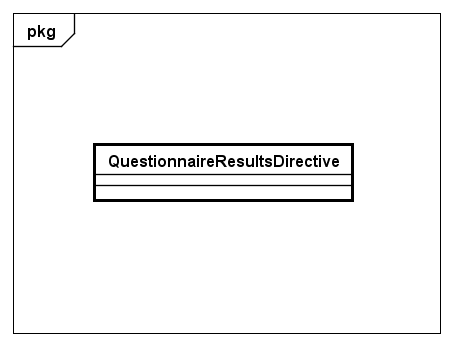
\includegraphics[scale=0.80,keepaspectratio]{UML/Classi/Front-End/QuizziPedia_Front-end_Directives_QuestionnaireResultsDirective.png}
	\caption{QuizziPedia::Front-End::Directives::QuestionnaireResultsDirective}
\end{figure} 
\FloatBarrier

\begin{itemize}
	\item \textbf{Descrizione}: rappresenta il componente grafico che permette all'utente autenticato pro di vedere i risultati di chi ha compilato il questionario. Tale componente è contenuto nella lista dei questionari abilitati alla compilazione. \'E possibile accedere alla lista dei risultati azionando l'evento ad esso collegato;
	\item \textbf{Utilizzo}: viene utilizzato per visualizzare i questionari abilitati alla compilazione e permettere all'utente di accedere alle statistiche ad essi associati;
	\item \textbf{Relazioni con altre classi}: 
	\begin{itemize}
		\item \textit{IN} \texttt{QuestionnaireManagementView}: view principale per la gestione dei questionari; 
		\item \textit{IN} \texttt{QuizEventController}: questa classe permette di reagire ai comandi dell'utente durante la gestione dei suoi questionari;
		\item \textit{IN} \texttt{LangModel}: rappresenta il modello delle informazioni per la giusta traduzione dell'applicazione.
	\end{itemize}
	\item \textbf{Attributi}: 
	\begin{itemize}
		\item {+ resultsButton: String} \\ Attributo che viene utilizzato per visualizzare la giusta traduzione della \textit{label\ped{G}} per il bottone di visualizzazione dei questionari, in italiano o in inglese;
		\item \texttt{+ controller: String} \\ Stringa contenente il nome del controller della direttiva;
		\item \texttt{+ restrict: String} \\ Stringa che permette di definire le modalità di inserimento della direttiva all'interno della pagina;
		\item \texttt{+ scope: Scope} \\ Oggetto scope interno della direttiva, contiene le funzionalità per gestire i dati presenti all'interno;
		\item \texttt{+ templateUrl: String} \\ Stringa contenente il percorso del file \textit{HTML\ped{G}} che contiene la direttive.
	\end{itemize} 
\end{itemize}
